\documentclass[9.5pt,a4paper]{article}
\usepackage[margin=1.65cm,top=1.4cm,bottom=1.52cm]{geometry}
\usepackage[T1]{fontenc}
\usepackage[utf8]{inputenc}
\usepackage{lmodern,microtype,graphicx,booktabs,amsmath,amssymb,xcolor,hyperref,array}
\usepackage[font=footnotesize,labelfont=bf]{caption}
\definecolor{ink}{HTML}{17243C}
\definecolor{accent}{HTML}{147D8C}
\definecolor{muted}{HTML}{526175}
\hypersetup{colorlinks=true,urlcolor=accent}
\setlength{\parindent}{0pt}
\setlength{\parskip}{3pt}
\setlength{\tabcolsep}{5pt}
\renewcommand{\arraystretch}{1.09}
\newcommand{\subhead}[1]{\vspace{5pt}{\color{ink}\bfseries\large #1}\vspace{1pt}\par}
\newcommand{\smhead}[1]{{\color{accent}\bfseries #1}}
\pagestyle{plain}
\begin{document}
\begin{center}
{\Large\bfseries\color{ink} Identifying Nonlinear Dynamical Systems with Generative Recurrent Networks}\\[-1pt]
{\normalsize\color{muted} Interim Progress Report \quad | \quad 8 December 2026 \quad | \quad Team 15}\\[3pt]
{\small Rub\'en Puyuelo, Alexis Usero and Mario Serrano}\\[-2pt]
{\footnotesize Dynamical Systems in Machine Learning, West University of Timi\c{s}oara}
\end{center}
\vspace{-2pt}
\hrule height 0.7pt
\vspace{5pt}

\smhead{Research question.} To what extent can piecewise-linear recurrent neural network state-space models (PLRNN-SSMs) identify and autonomously reproduce nonlinear dynamics, compared with linear dynamical state-space models (LDS-SSMs), and how does hemodynamic filtering affect an extension toward fMRI?

\subhead{1. Motivation and current scope}
Chaotic or oscillatory systems may be predictable over a short horizon even when the learned model does not reproduce the geometry of their long-term dynamics. Koppe \emph{et al.}~[1] address this distinction with a generative PLRNN and a probabilistic observation model. We have implemented a \emph{simplified, independent Python research prototype} for two synthetic benchmarks (van der Pol and Lorenz), a linear baseline, stability-aware refinement, and synthetic BOLD-like observations. The application to genuine human fMRI remains future work.

\subhead{2. Models and experimental design}
For the PLRNN, the latent transition and the standard observation decoder are
\begin{equation}
z_t=A z_{t-1}+W\,\mathrm{ReLU}(z_{t-1})+b+\epsilon_t,
\qquad
x_t=B\,\mathrm{ReLU}(z_t)+\eta_t.
\label{eq:plrnn}
\end{equation}
Here $A$ is diagonal, $W$ has a zero diagonal, and $\epsilon_t,\eta_t$ are noise terms. The LDS instead uses linear transition and observation mappings. Its latent states are inferred by Kalman filtering/smoothing and its parameters by expectation--maximization. Our PLRNN estimates a latent path with an alternating joint maximum-a-posteriori (MAP) procedure and progressive process-consistency weighting; this is \textbf{not} the original paper's full Laplace--EM inference or annealing algorithm.

\smhead{Data and evaluation.} Each benchmark provides 1,000 standardized simulated samples: 700 for fitting and 300 held out, with Gaussian \emph{observation} noise. We evaluate short-horizon forecast mean squared error (MSE) and independently generated free-running trajectories. Long-run comparison uses histogram Jensen--Shannon divergence (JSD; lower is better), stability diagnostics, and qualitative attractor plots. Our JSD is not the normalized $\mathrm{KL}$ score in~[1]. For robustness, three trained PLRNN seeds are evaluated from three training-derived initial states each; these are \emph{three fits, not nine independent fits}.

\subhead{3. Initial benchmark results}
\begin{center}
\begin{tabular}{@{}lccccc@{}}
\toprule
& \multicolumn{2}{c}{Held-out 10-step MSE$^{a}$} & \multicolumn{2}{c}{Long-run median JSD$^{b}$}\\
Benchmark & LDS & PLRNN & Matched-$M$ LDS & PLRNN\\
\midrule
van der Pol & 0.3131 & \textbf{0.1445} & 0.4996 & \textbf{0.4312}\\
Lorenz & 2.9486 & \textbf{0.8683} & 0.5891 & \textbf{0.4218}\\
\bottomrule
\end{tabular}
\end{center}
{\footnotesize $^{a}$Initial phase-3 comparison, seed 42: PLRNN latent sizes $M=8/12$ and LDS $M=2/3$; different inference procedures, so this is \emph{illustrative}, not parameter-matched. $^{b}$Phase-4 autonomous evaluation: LDS and PLRNN have matched latent sizes but not parameter counts; 3 PLRNN fits $\times$ 3 related initializations versus 3 LDS fits.}

The PLRNN forecasts more accurately in these initial experiments and generally occupies a more plausible region of state space. However, the original PLRNN often learns a distorted van der Pol cycle and \emph{does not} reconstruct the Lorenz chaotic butterfly. Thus lower forecast MSE cannot be interpreted as faithful dynamical identification.

\begin{center}
\vspace{1pt}
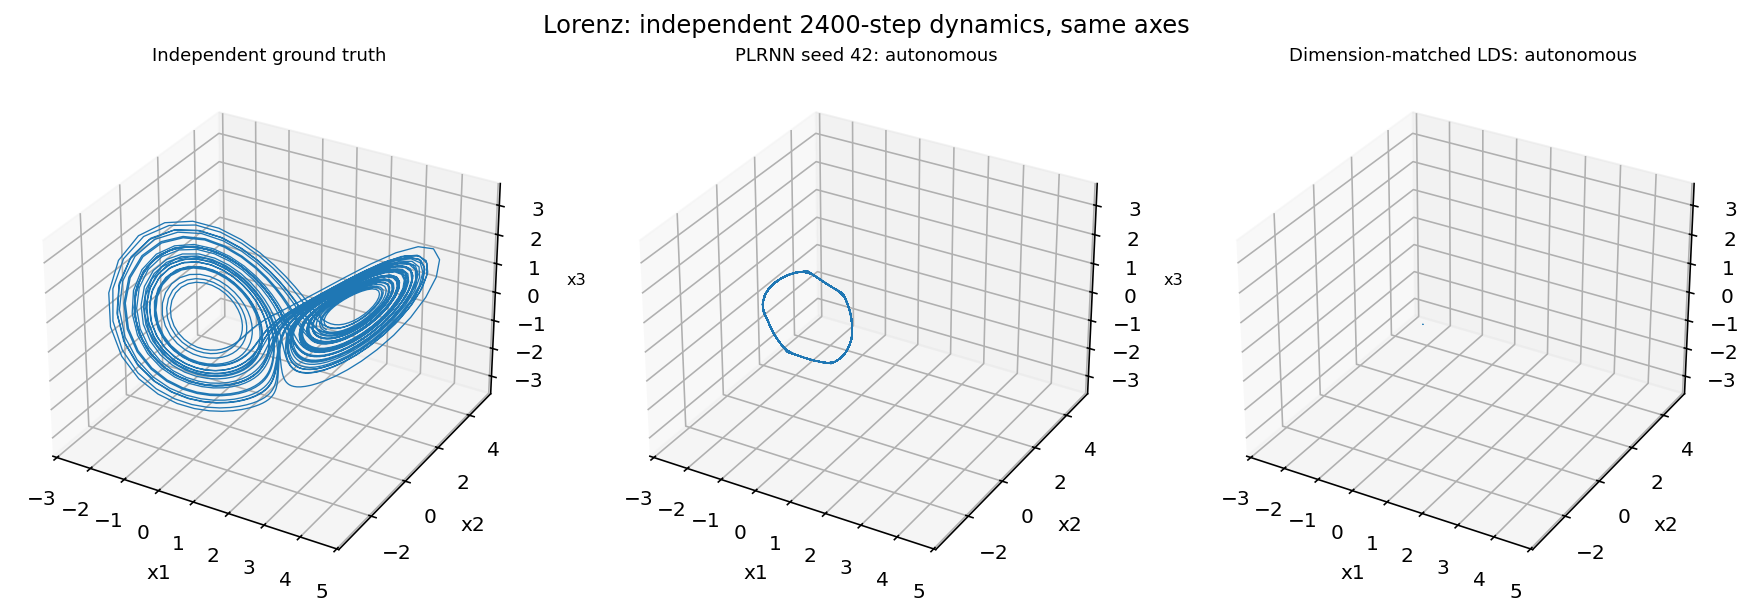
\includegraphics[width=.66\linewidth]{figures/lorenz_long_rollout.png}\\[-4pt]
{\footnotesize\textbf{Figure 1.} Lorenz reference, PLRNN and matched-$M$ LDS, all free-running.}
\end{center}

\newpage
\vspace*{-8pt}
\subhead{4. Stability-aware multi-step refinement}
We added a train-only, truncated multi-step forecast loss for the PLRNN transition and selected among interpolated parameter updates using training-data dynamical diagnostics. Selection rejects unstable autonomous trajectories; independent ODE trajectories are used only for post-selection evaluation. The approach is exploratory and does not reproduce the original algorithm.

\begin{center}
\begin{tabular}{@{}lrrrrrr@{}}
\toprule
& \multicolumn{3}{c}{van der Pol JSD} & \multicolumn{3}{c}{Lorenz JSD}\\
Training seed & 42 & 7 & 21 & 42 & 7 & 21\\
\midrule
Before & 0.431 & 0.500 & 0.202 & 0.458 & 0.420 & 0.422\\
After  & \textbf{0.059} & \textbf{0.127} & \textbf{0.049} & \textbf{0.394} & 0.420 & 0.422\\
\bottomrule
\end{tabular}
\end{center}
The van der Pol geometric discrepancy decreased for all three seeds. For Lorenz, one checkpoint improved modestly and two retained their original parameters; the resulting trajectories still lack a faithful chaotic attractor.

\begin{figure}[h!]
\centering
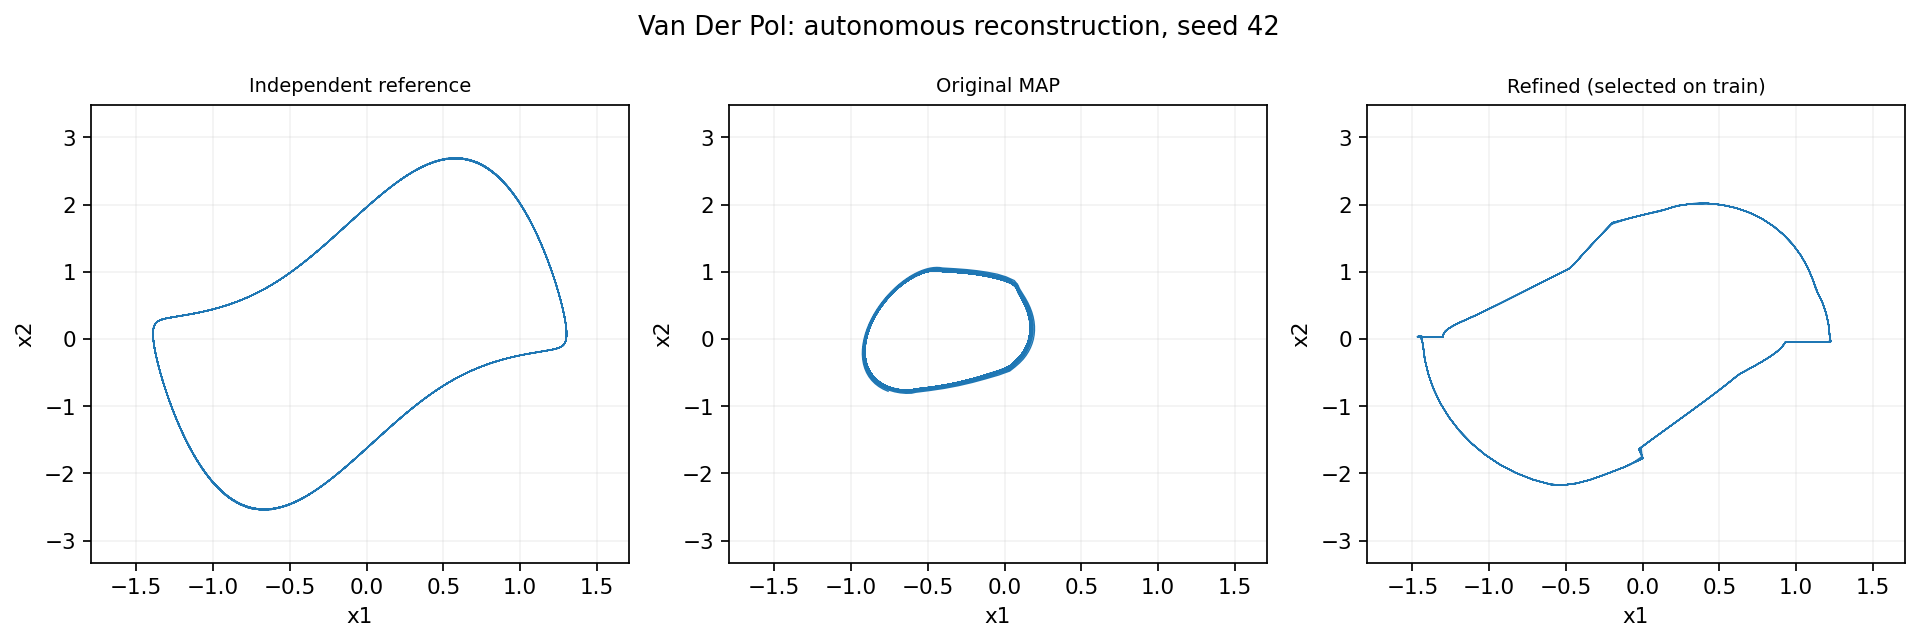
\includegraphics[width=.93\linewidth]{figures/van_der_pol_refinement.png}
\vspace{-5pt}
\caption{Independent van der Pol reference (left), original PLRNN (middle), and refined PLRNN (right); selected seed 42. A better cycle is recovered, but this is not proof of exact system identification.}
\end{figure}
\vspace{-7pt}
\subhead{5. Synthetic BOLD / hemodynamic observation extension}
To examine the relevance to fMRI without claiming to analyze human recordings, we transformed standardized ODE trajectories into \emph{BOLD-like synthetic signals} using a fixed causal double-gamma hemodynamic response function (HRF):
\[
y_t=B\sum_{k=0}^{L-1}h_k z_{t-k}+\eta_t.
\]
In a controlled \emph{known-state (oracle)} decoder comparison, the held-out clean-BOLD MSE was $1.1\times10^{-5}$ versus $0.1211$ on van der Pol, and $8.35\times10^{-5}$ versus $0.5503$ on Lorenz (HRF-aware versus instantaneous). Because the synthetic data were generated using the same known HRF, this verifies the observation-model specification; it is \emph{not} evidence of latent-state recovery.

With latent paths \emph{unknown}, the approximate HRF-aware PLRNN attained autonomous BOLD JSD $0.123$ versus $0.238$ for the instantaneous comparator on van der Pol (one seed). On Lorenz its autonomous rollout diverged, so no full-horizon JSD is reported. These findings separate correct signal filtering from the harder problem of discovering the underlying dynamical law.

\subhead{6. Limitations and next steps}
The current study is small and exploratory: synthetic data only; simplified MAP inference instead of full probabilistic EM; no matched model parameter counts or formal significance testing; reference dynamics may differ from real neuronal processes; no nuisance regressors or empirical task inputs. Our benchmarks inject observation rather than the original paper's process noise, and the illustrative HRF time scale is not physiologically calibrated.

\smhead{Before final submission (19 January 2027):} perform additional train/validation-segregated repeats; report stability and failures as well as successes; investigate more faithful latent inference or stable training for Lorenz; assess whether documented, preprocessed ROI-level human fMRI data can be incorporated; and finalize reproducible code, interpretation, and a 15-minute presentation.

\vspace{1pt}\hrule\vspace{2pt}
{\footnotesize \textbf{Reference.} G. Koppe \emph{et al.}, ``Identifying nonlinear dynamical systems via generative recurrent neural networks with applications to fMRI,'' \emph{PLOS Computational Biology}, 15(8):e1007263, 2019. \url{https://doi.org/10.1371/journal.pcbi.1007263}.}
\end{document}
